\documentclass[a4paper,12pt]{article}
\usepackage{polski}
\usepackage[utf8]{inputenc}
\usepackage[OT4]{fontenc}
\usepackage{mathtools}
\usepackage{float}
\usepackage{graphicx}
\usepackage{multirow}
\usepackage{listings}
\usepackage{hyperref}
\usepackage[table,xcdraw]{xcolor}

\begin{document}

%-------------------------------------------------------
%					### TYTUŁOWA ###	

\begin{center}
	\LARGE STRUKTURY DANYCH I ZŁOŻONOŚĆ OBLICZENIOWA\\
	\Large Zadanie projektowe nr 2
	
	\begin{table}[H]
		\centering
		\begin{tabular}{|c|}
			\hline
			\textbf{Temat:}                                                                                                                               \\ \hline
			\begin{tabular}[c]{@{}c@{}}Badanie efektywności algorytmów grafowych.\end{tabular} \\ \hline
			\textbf{Autor:}                                                                                                                               \\ \hline
			Dawid Waligórski                                                                                                                             \\ \hline
			\textbf{Termin zajęć:}                                                                                                                        \\ \hline
			Wtorek, godz. 15.15, TP                                                                                                                      \\ \hline
		\end{tabular}
	\end{table}
	
\end{center}

\newpage

\tableofcontents

\newpage

%-------------------------------------------------------
%	CEL ZADANIA PROJEKTOWEGO
\section{Założenia projektowe:}

\subsection{Cele projektu:}
Celem projektu była implementacja algorytmów grafowych wraz z niezbędnymi do ich działania strukturami danych w języku C++. Kluczowym było również dokonanie pomiaru czasów wykonywania się wspomnianych algorytmów na grafach o różnych reprezentacjach, rozmiarach (liczba wierzchołków) oraz gęstościach (liczba krawędzi). Badanymi algorytmami były:
\begin{itemize}
	\item Algorytm Prima (problem wyznaczenia MST)
	\item Algorytm Kruskala (problem wyznaczenia MST)
	\item Algorytm Dijkstry (problem wyszukiwania najkrótszych ścieżek)
	\item Algorytm Bellmana-Forda (problem wyszukiwania najkrótszych ścieżek)
\end{itemize}
\vspace{5mm}

\noindent
Tworzona aplikacja z konsolowym interfejsem użytkownika, poza możliwością przeprowadzenia eksperymentów miała oferować również opcję sprawdzenia poprawności zaimplementowanych algorytmów za pomocą dedykowanych menu.\\

\noindent
Szczegółowe założenia tyczące się poszczególnych algorytmów zostały zawarte w odpowiadających im rozdziałach.

\subsection{Grafy:}
Założono, że wierzchołki grafu będą identyfikowane przez kolejne, nieujemne liczby całkowite (typ \it unsigned int\rm). Do przechowywania wartości krawędzi wybrano znakowany, 4-bajtowy typ całkowity (\it int\rm). W zależności od wybranego problemu mogły być one skierowane (najkrótsza ścieżka) lub nieskierowane (MST).\\

\noindent
Badane algorytmy otrzymać miały swoje odpowiedniki dla dwóch różnych sposobów reprezentacji grafu. Pierwszy z nich zakładał użycie macierzy sąsiedztwa. Drugi korzystać miał ze zbioru połączonych list sąsiadów. W wypadku macierzy sąsiedztwa, zamiast tradycyjnej, binarnej informacji o istnieniu krawędzi między wierzchołkami, miała ona zawierać informację o wadze krawędzi. Brak połączenia w tej strukturze był oznaczany za pomocą specjalnej, zarezerwowanej wartości NO\_CONNECTION (wartość minimalna typu \it int\rm).\\

\noindent
Dodatkowo możliwym miało być wczytanie grafu z pliku (np. tekstowego). Pierwsza linia w takim pliku definiować miała liczbę wierzchołków, krawędzi, a także wierzchołki początkowy i końcowy (wykorzystywane przy niektórych algorytmach). W kolejnych liniach znajdować się miały dane na temat kolejnych krawędzi grafu w konwencji: wierzchołek początkowy, wierzchołek końcowy, waga.

%-------------------------------------------------------
%	METODA POMIAROWA
\section{Metoda pomiarowa:}

\subsection{Środowisko pomiarowe:}
Pomiary przeprowadzano na komputerze stacjonarnym z zainstalowanym systemem Windows 10 (wersja 64-bitowa). Częstotliwość taktowania zegara procesora wynosiła 3,60GHz. Ilość pamięci operacyjnej wynosiła 16GB. W trakcie pomiarów na maszynie działały jedynie niezbędne do funkcjonowania systemu operacyjnego procesy. Aplikacja mierząca działała w domyślnym trybie przydziału zasobów komputera. Była ona skompilowana za pomocą narzędzia \it g++ \rm na poziomie optymalizacji O3. 

\subsection{Pomiary wykonywane w programie:}

\subsubsection{Narzędzie pomiarowe:}
W pomiarach czasu wykorzystano specjalną klasę \it Timer\rm. Instancja wspomnianej klasy działała na zasadzie stopera, mierząc czas pomiędzy wywołaniami swoich metod \it start() \rm oraz \it stop()\rm. Precyzja prowadzonego nią pomiaru była rzędu 0,1 mikrosekundy ($10^{-7}s$). Przykład użycia \it Timer \rm został zamieszczony na rysunku \ref{timer-przyklad}.
\begin{figure}[H]
	\centering
	\caption{\centering Przykład użycia klasy \it Timer \rm do pomiaru czasu wykonania algorytmu Bellmana-Forda.}
	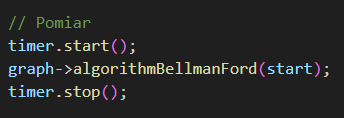
\includegraphics[width=7cm]{fig2.png}
	\label{fig.timer-przyklad}
\end{figure}

\subsubsection{Przebieg pomiaru:}
Pomiary czasu wykonywania algorytmów zostały wkomponowane jako jedne z opcji możliwych do wyboru z poziomu aplikacji projektowej (rys. \ref{fig.opcja-badanie}). W wypadku wybrania takiej opcji aplikacja dawała użytkownikowi opcję wyboru algorytmu, który miał zostać przebadany. Następnie wykonywany był właściwy pomiar, dzielący się na 40 faz. Każda faza wyróżniała się inną kombinacją parametrów używanego w pomiarach grafu. Owe parametry oraz ich dopuszczalne wartości zamieszczono w tabeli \ref{tab-parametry}. W trakcie jednej fazy wykonywano łącznie 100 prób. Dla każdej z osobna generowano nową, losową instancję grafu (odpowiedniego dla danego algorytmu). Później za pomocą klasy \it Timer \rm dokonywano pomiaru czasu wykonywania wybranego algorytmu. W końcu dane o próbie były zapisywane w specjalnej strukturze, która po zakończeniu się danej fazy była zapisywana do pliku \it *.csv \rm w formie jednego z jego z rekordów. Pola takiego rekordu została zamieszczona w tabeli \ref{tab.wynik-pomairu}.
\begin{figure}[H]
	\centering
	\caption{\centering Menu główne, zawierające opcję przeprowadzenia pomiarów.}
	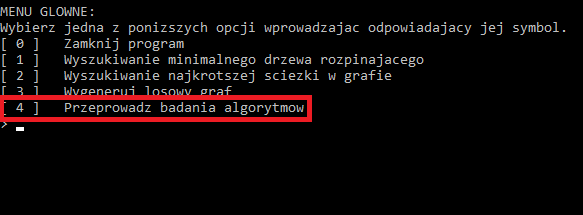
\includegraphics[width=12cm]{fig1.png}
	\label{fig.opcja-badanie}
\end{figure}

\begin{table}[H]
	\centering
	\caption{\centering Tabela zawierające parametry grafów używanych w poszczególnych fazach badania wraz z ich dopuszczalnymi wartościami.}
	\label{tab-parametry}
	\begin{tabular}{|l|c|c|c|}
		\hline
		\textbf{Parametr:}  & Reprezentacja                                                             & Rozmiar                                                             & Gęstość                                                                                                              \\ \hline
		\textbf{Opis:}     & \begin{tabular}[c]{@{}c@{}}Sposób \\ reprezentacji \\ grafu.\end{tabular} & \begin{tabular}[c]{@{}c@{}}Liczba \\ wierzchołków.\end{tabular}     & \begin{tabular}[c]{@{}c@{}}Stosunek liczby krawędzi \\ grafu do jego \\ maksymalnej \\ liczby krawędzi.\end{tabular} \\ \hline
		\textbf{Wartości:} & \begin{tabular}[c]{@{}c@{}}listowa\\ macierzowa\end{tabular}              & \begin{tabular}[c]{@{}c@{}}100\\ 200\\ 300\\ 400\\ 500\end{tabular} & \begin{tabular}[c]{@{}c@{}}25\%\\ 50\%\\ 75\%\\ 99\%\end{tabular}                                                    \\ \hline
	\end{tabular}
\end{table}

\begin{table}[H]
	\centering
	\label{tab.wynik-pomairu}
	\caption{\centering Tabela zawierająca strukturę rekordu pliku \it *.csv\rm, zawierającego wyniki pomiarów.}
	\begin{tabular}{|l|l|}
		\hline
		\textbf{Algorytm}      & Inicjał odpowiadający badanemu algorytmowi. \\ \hline
		\textbf{Reprezentacja} & Typ reprezentacji przebadanego grafu.       \\ \hline
		\textbf{Rozmiar}       & Rozmiar przebadanego grafu.                 \\ \hline
		\textbf{Gęstość}       & Gęstość przebadanego grafu.                 \\ \hline
		\textbf{Czas}          & Zmierzony czas.                             \\ \hline
	\end{tabular}
\end{table}

\subsubsection{Generowanie grafu:}
Za generowanie losowych instancji grafów, używanych w badaniach odpowiedzialna była klasa \it GraphGenerator\rm. Była ona paremetryzowana wartościami takimi jak:
\begin{itemize}
	\item Typ reprezentacji grafu
	\item Liczba wierzchołków
	\item Informacja o skierowaniu krawędzi
	\item Gęstość grafu
	\item Informacja o dopuszczalności wystąpienia ujemnych wag krawędzi
\end{itemize}
\vspace{5mm}

\noindent
Tak duża gama parametrów pozwoliła na generowanie grafów dobrze przystosowanych do każdego z zaimplementowanych algorytmów (np. zabraniając generowania się ujemnych krawędzi w wypadku algorytmu Dijkstry).\\

\noindent
Najważniejszym i najbardziej wymagającym zadaniem powierzonym omawianej klasie było generowanie losowego zbioru krawędzi dla tworzonego grafu. Było ono wykonywane w dwóch etapach. W pierwszym generowane, a następnie umieszczane w tablicy były wszystkie, możliwe dla danego typu grafu (skierowany/nieskierowany) krawędzie. Drugi etap polegał na wybraniu z uzyskanej kolekcji krawędzi losowego podzbioru o wielkości podyktowanej przez parametr gęstości grafu. Odbywało się to poprzez kolejne losowania indeksu z wygenerowanej w etapie pierwszym tablicy, stale pomniejszanej o już wybrane krawędzie. 

\subsection{Przetworzenie wyników w arkuszu kalkulacyjnym:}

%-------------------------------------------------------
%	WYZNACZANIE MINIMALNEGO DRZEWA SPINAJĄCEGO
\section{Wyznaczanie MST:}

\subsection{Algorytm Prima:}

\subsection{Algorytm Kruskala:}

\subsection{Wyniki pomiarów:}

\subsection{Analiza wyników pomiarów:}

%-------------------------------------------------------
%	WYZNACZANIE MINIMALNEGO DRZEWA SPINAJĄCEGO
\section{Wyznaczanie najkrótszej ścieżki:}

\subsection{Algorytm Dijkstry:}

\subsection{Algorytm Bellmana-Forda:}

\subsection{Wyniki pomiarów:}

\subsection{Analiza wyników pomiarów:}

%-------------------------------------------------------
%	WNIOSKI
\section{Wnioski:}

\end{document}